% !TeX spellcheck = es_ES
\documentclass[a4paper, 12pt, spanish]{report}
\usepackage[spanish]{babel}
\selectlanguage{spanish}
\usepackage[utf8]{inputenc} %Se usa para que admita texto con tildes
\usepackage[T1]{fontenc}	%Se usa para que admita texto con tildes
\usepackage{amsmath}
\usepackage{listings}
\usepackage{color}	%Se usa para definir colores en el documento
\usepackage{ulem}	%Se usa para poner código en el documento.
\usepackage{bm}	%Se usa para hacer expresiones matemáticas en negrita
\usepackage[a4paper,vmargin=2cm,hmargin=1cm]{geometry}
\usepackage{diagbox}	%Se usa para hacer la linea diagonal dentro de la celda de una tabla

\usepackage{mathtools}	%se usa para hacer recuadros dentro de align con \Aboxed{}
\usepackage{chngcntr}	%se usa para resetear el contador de ecuaciones

\usepackage{empheq}		%se usa para hacer ecuaciones alineadas dentro de una caja.
\newcommand*\widefbox[1]{\fbox{\hspace{2em}#1\hspace{2em}}}

\usepackage{alltt}
\usepackage{pgfplots}
\usepackage{multicol}
\usepackage{caption}
\usepackage{subcaption}
\usepackage{float}
\usepackage{multicol}

%configuracion de package {chngcntr}
\counterwithin*{equation}{section}
\counterwithin*{equation}{subsection}

%Definición de colores para el documento
\definecolor{dkgreen}{rgb}{0,0.6,0}
\definecolor{gray}{rgb}{0.5,0.5,0.5}
\definecolor{mauve}{rgb}{0.58,0,0.82}
%Definicion de ulem para el código
\lstset{
	language=PHP,
	aboveskip=3mm,
	belowskip=3mm,
	showstringspaces=false,
	columns=flexible,
	basicstyle={\ttfamily},
	numbers=left,
	numberstyle=\tiny\color{gray},
	keywordstyle=\color{blue},
	commentstyle=\color{dkgreen},
	stringstyle=\color{mauve},
	breaklines=true,
	breakatwhitespace=true,
	tabsize=3
}

\title{Secciones y Capítulos}
\author{Juan Aparicio}
\begin{document}
\begin{titlepage}
	\centering
	
\includegraphics[width=0.15\textwidth]{imagenes/logo.png}\par\vspace{1cm}
	{\scshape\LARGE Taller de Informática\par}
	\vspace{1cm}
	{\scshape\Large Entrega\par}
	\vspace{1.5cm}
	{\huge\bfseries Documentación\par}
	\vspace{2cm}
	{\Large\itshape Juan Aparicio\par}
	\vfill
	supervisado por \par
	Carolina 		
	\vfill
	% Bottom of the page
	{\large 12, 2017\par}
\end{titlepage}

%Segunda página
\tableofcontents
\newpage

%Tercera página
%Acá van las secciones, etc

\chapter{Instalación}
\begin{enumerate}
	\item Primero lo que hay que hacer es asegurarse tener apache, php 5 o mayor, y MySQL instalados.
	\item Una vez instalados los programas, copiar el contenido de la carpeta \verb|administracion_gimnasio| a la carpeta que contenga las páginas de apache.
	\item Luego hay que ejecutar el script \verb|sist_gim.sql|, el cual creará la base de datos \verb|Gimnasio| en donde se almacenará toda la información del sistema.
	\item Luego de ejecutar el script queda finalizada la instalación del sistema, lista para su uso.
\end{enumerate}

\chapter{Manual de uso}
\section{Usuarios}
\par En esta sección se indicará como llevar a cabo la administración de los usuarios del sistema.
\subsection{Registro}
\par Primero ir a la sección \verb|Usuarios| en la barra de navegación y dentro de esta sección elegir \verb|Registro Usuario|. Esto desplegará la siguiente pantalla.
\begin{figure}[H]
	\centering
	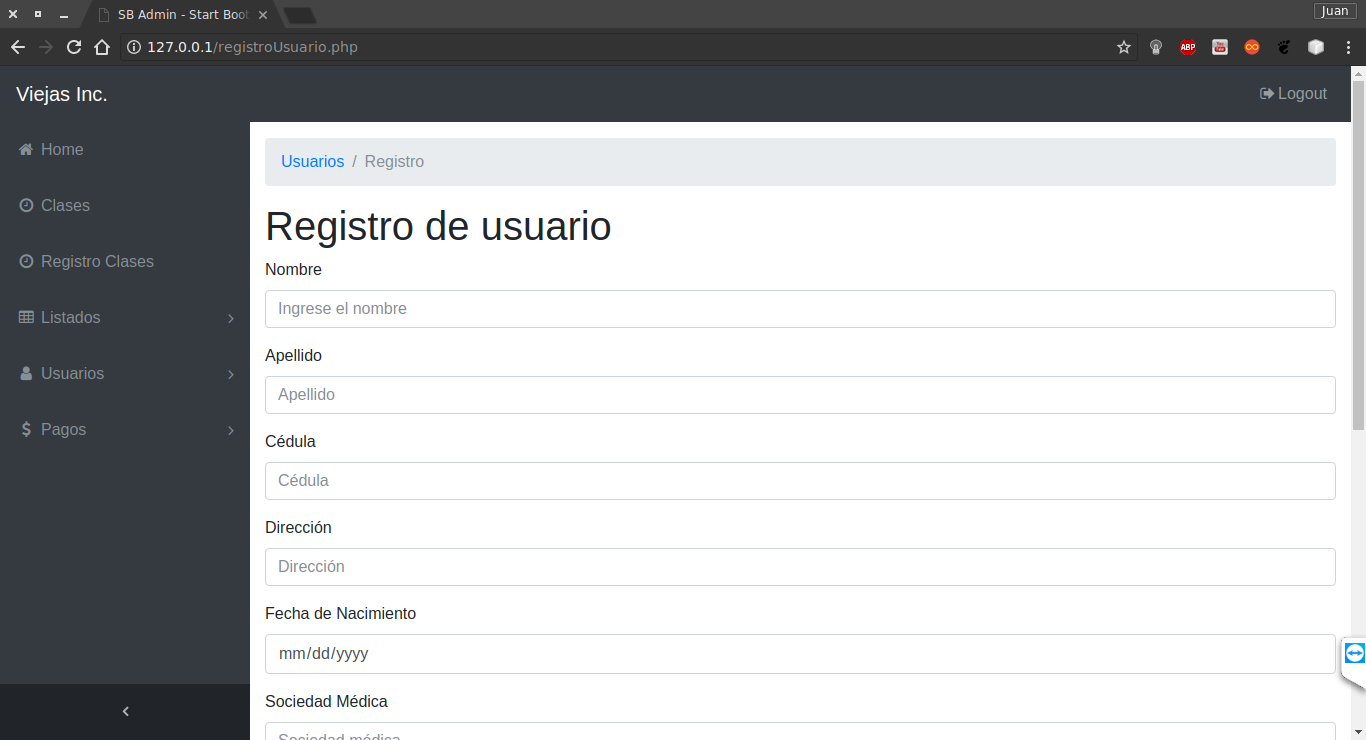
\includegraphics[width=\linewidth]{imagenes/registro}
	\label{fig:registro}
\end{figure}
\par Luego de ingresados los datos (la fecha tiene que tener formato mes-dia-año), presionar el botón ingresar al final de la página.
\begin{figure}[H]
	\centering
	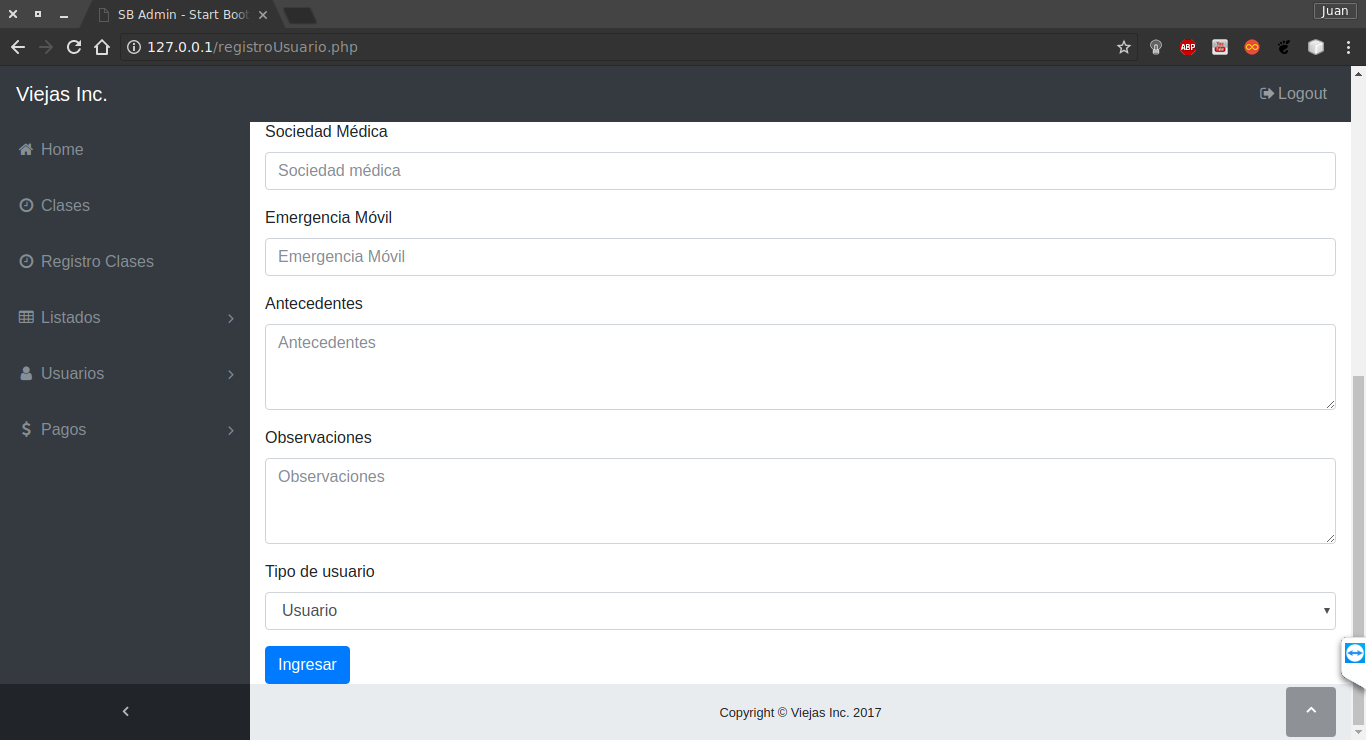
\includegraphics[width=\linewidth]{imagenes/registro_ingresar}
	\label{fig:registro_ingresar}
\end{figure}
\par Si el registro es exitoso, se mostrara una mensaje de confirmación, de lo contrario, se mostrará un mensaje con el error en cuestión.

\subsection{Modificación}
\par Primero ir a la sección \verb|Usuarios| en la barra de navegación y dentro de esta sección elegir \verb|Modificación Usuario|. Esto desplegará la siguiente pantalla.
\begin{figure}[H]
	\centering
	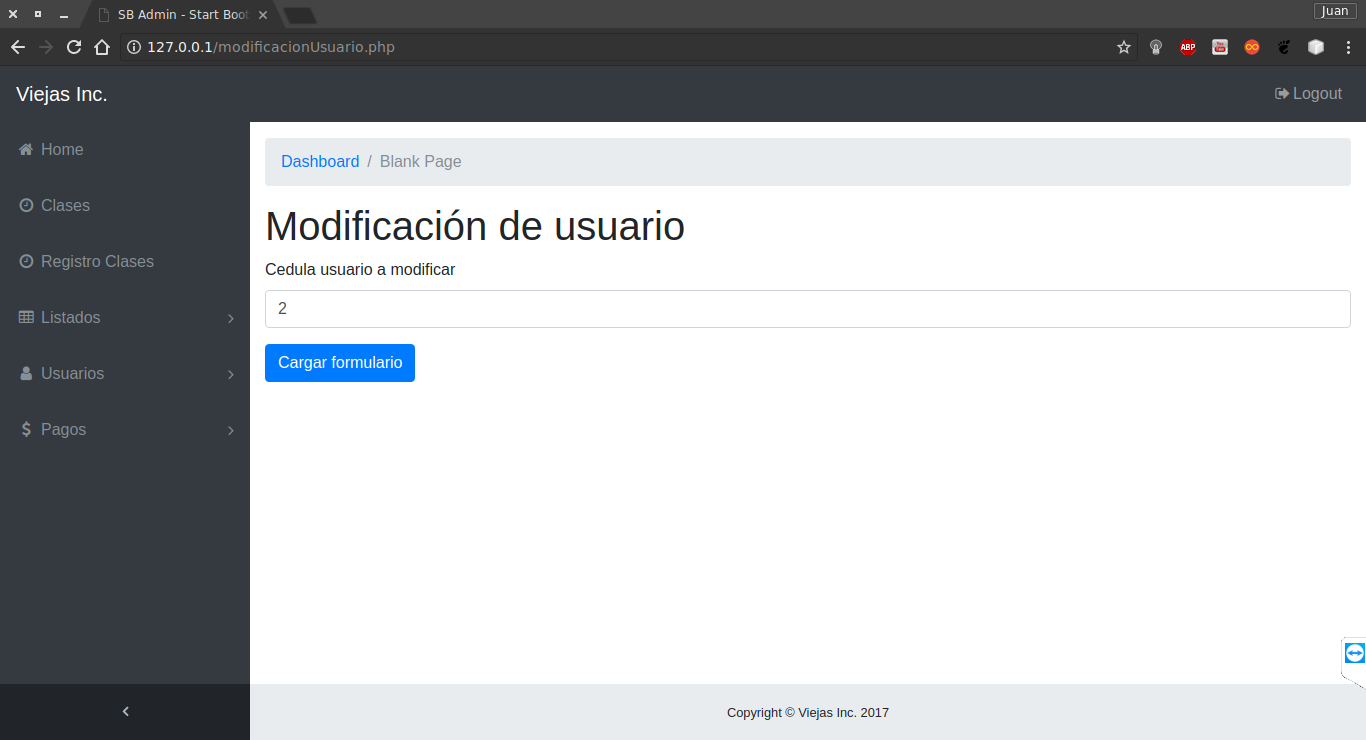
\includegraphics[width=\linewidth]{imagenes/us_mod_carg}
	\label{fig:usmodcarg}
\end{figure}
\par En esta pantalla se ingresa la cédula del usuario que se desea modificar y luego de ingresada la cédula, se cargará un formulario con los datos del usuario. Aquí se modifican los que se quiere y luego de modificar los datos deseados, se presiona el botón Modificar:
\begin{figure}[H]
	\centering
	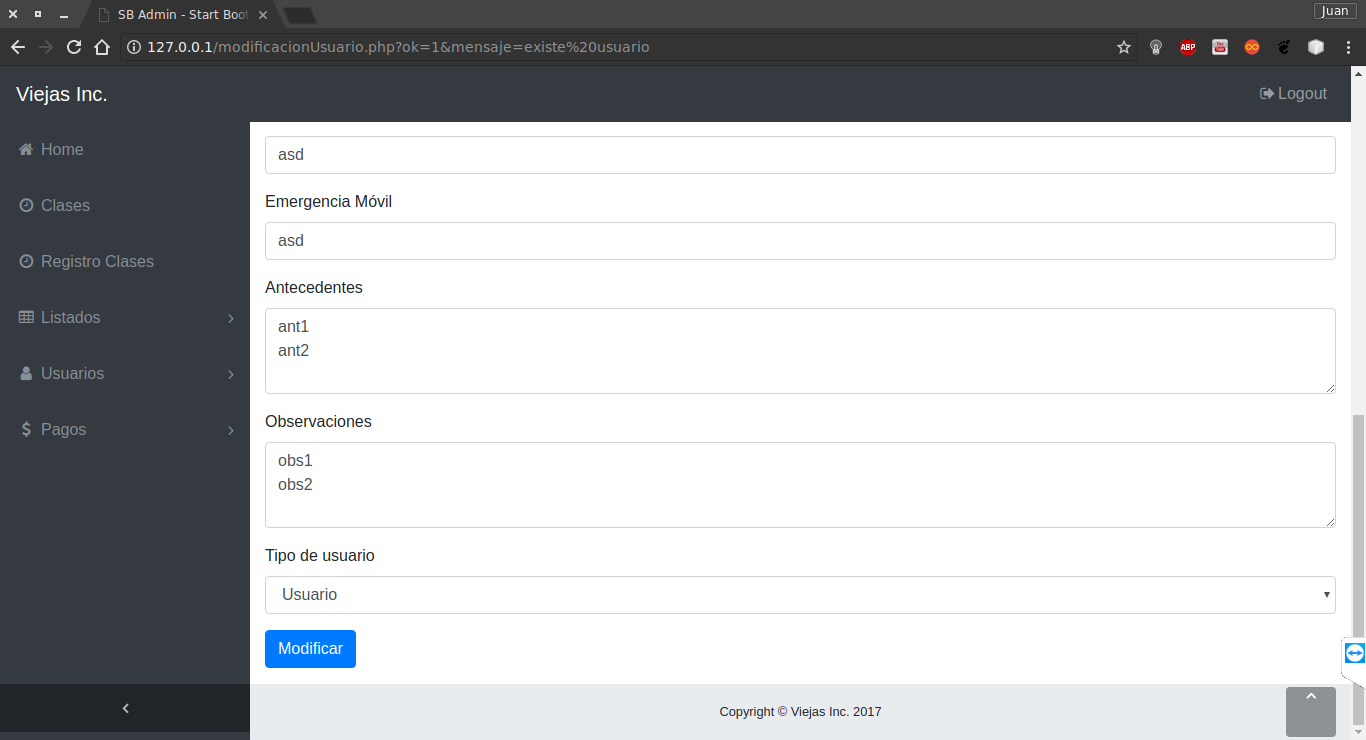
\includegraphics[width=\linewidth]{imagenes/us_mod_mod}
	\label{fig:usmodmod}
\end{figure}

\subsection{Baja (lógica)}
\par Primero ir a la sección \verb|Usuarios| en a barra de navegación, y dentro de esta sección elegir \verb|Baja Usuario|. Esta funcionalidad lo que hace es darle de baja a un usuario, sin embargo no lo borra permanentemente de la base de datos. Esto desplegará la siguiente pantalla:
\begin{figure}[H]
	\centering
	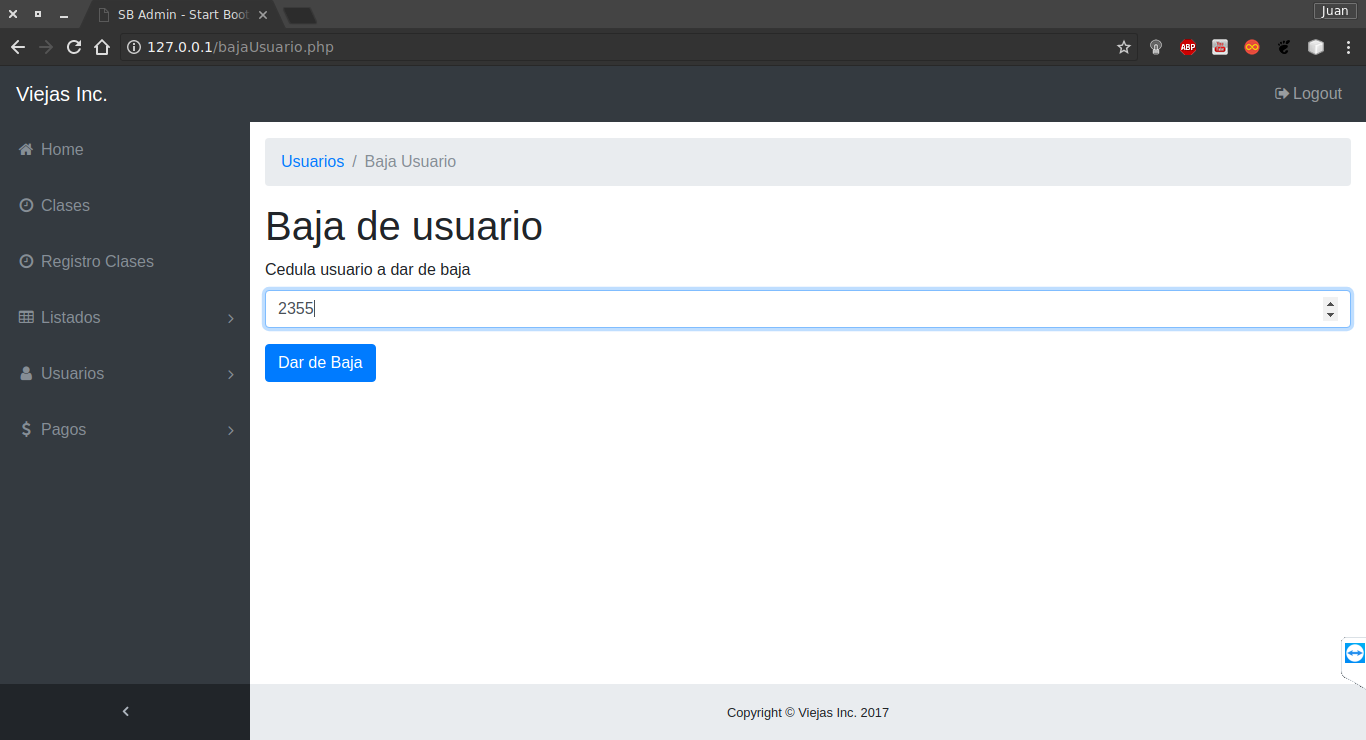
\includegraphics[width=\linewidth]{imagenes/us_baj_carg}
	\label{fig:usbajcarg}
\end{figure}
\par Aquí se ingresa la cédula del usuario que se desea dar de baja. Luego presionar el botón \verb|Dar de Baja|.
\par Si el usuario se dio de baja con éxito, aparecerá un mensaje de confirmación. De lo contrario un mensaje con el error en cuestión.

\subsection{Alta (lógica)}
\par Esta funcionalidad funciona igual que la Baja lógica. La diferencia es que esta es para darles de alta.
\subsection{Listado}
\par Primero ir a la sección \verb|Listados| en a barra de navegación, y dentro de esta sección elegir \verb|Listado de Usuarios|. Esto desplegará la siguiente pantalla:
\begin{figure}[H]
	\centering
	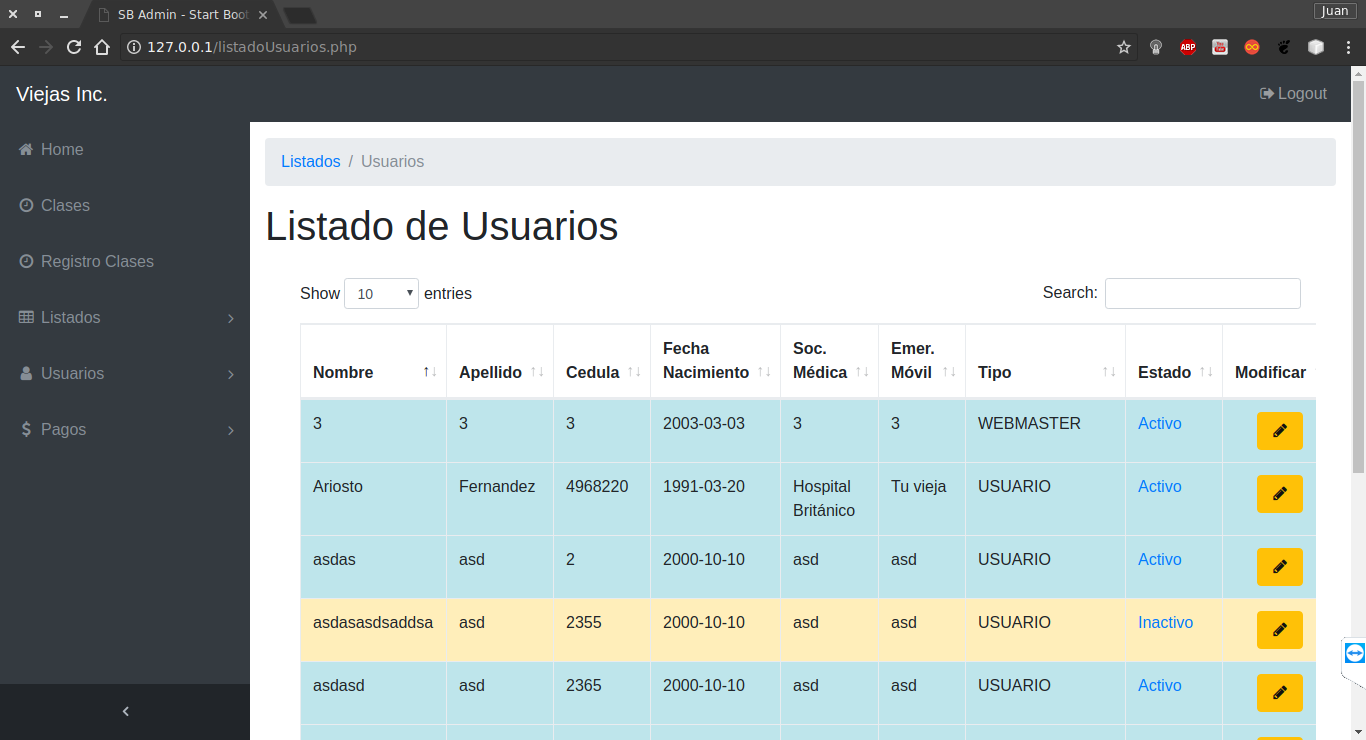
\includegraphics[width=\linewidth]{imagenes/us_list_comp}
	\label{fig:uslistcomp}
\end{figure}
\par En la tabla se muestra un listado de los usuarios con sus datos, una columna con un link que dice \verb|Activo| si el usuario esta dado de alta, y \verb|Inactivo| de lo contrario. Al apretar el link, se redireccionará a la seccion de baja/alta de usuario con la cédula del usuario ya cargada en el formulario. La columna modificar tiene un link que redirecciona a la página de modificación de usuario y carga la cédula de dicho usuario en el formulario. Por ultimo la columna \verb|Pago Atrasado| toma los valores \verb|Atrasado| si el usuario está atrasado en sus pagos o \verb|-| si el usuario se día con los pagos.
\par La barra de búsqueda busca el texto ingresado en todas las columnas. Si el texto ingresado se encuentra en algún campo del usuario, entonces aparecerá en el listado. Por ejemplo si se quiere buscar los usuarios que se encuentren atrasados en sus pagos, se ingresa el texto \verb|Atrasado| en la barra de búsqueda y aparecerán solo aquellos en la tabla:
\begin{figure}[H]
	\centering
	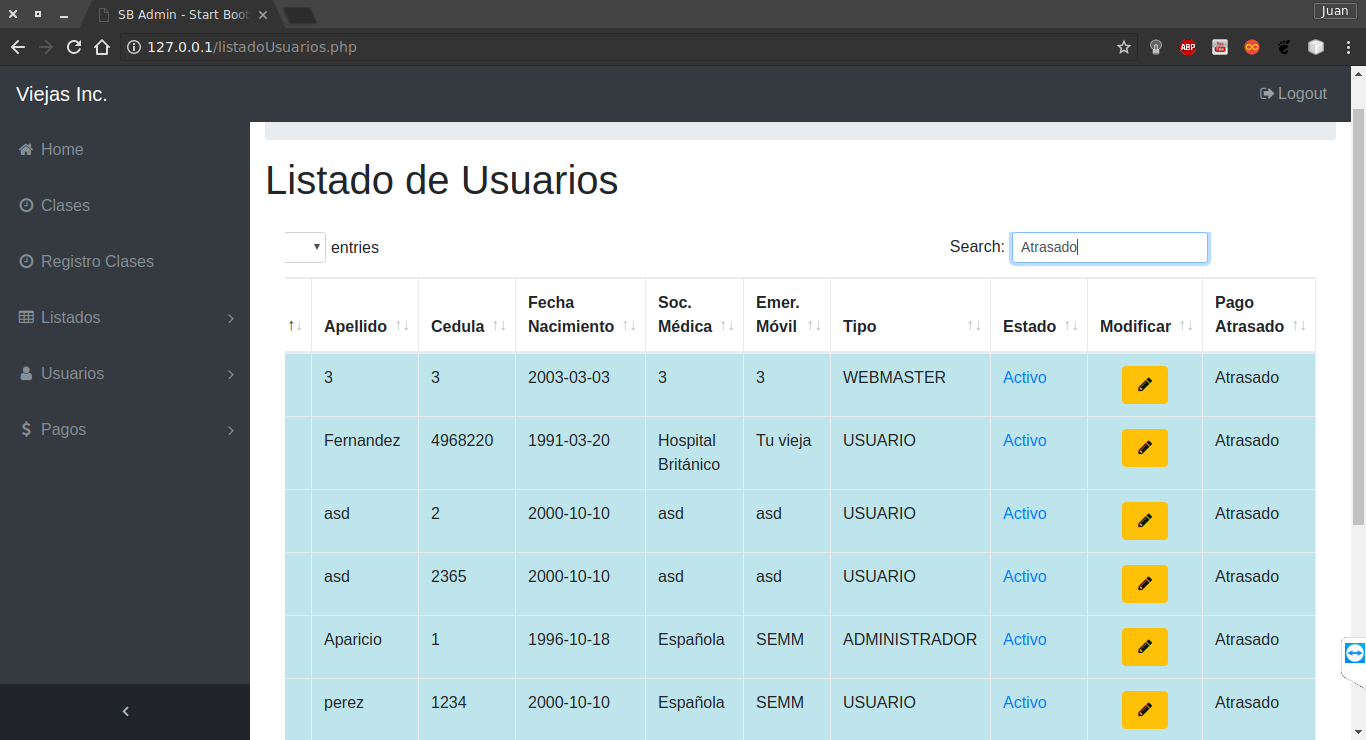
\includegraphics[width=\linewidth]{imagenes/us_list_atr}
	\label{fig:uslistatr}
\end{figure}

\newpage
\section{Pagos}
En esta sección se indicará como llevar a cabo la administración de los pagos del sistema.
\subsection{Registro}
\par Primero ir a la sección \verb|Pagos| en a barra de navegación, y dentro de esta sección elegir \verb|Registro Pago|. Esto desplegará la siguiente pantalla:
\begin{figure}[H]
	\centering
	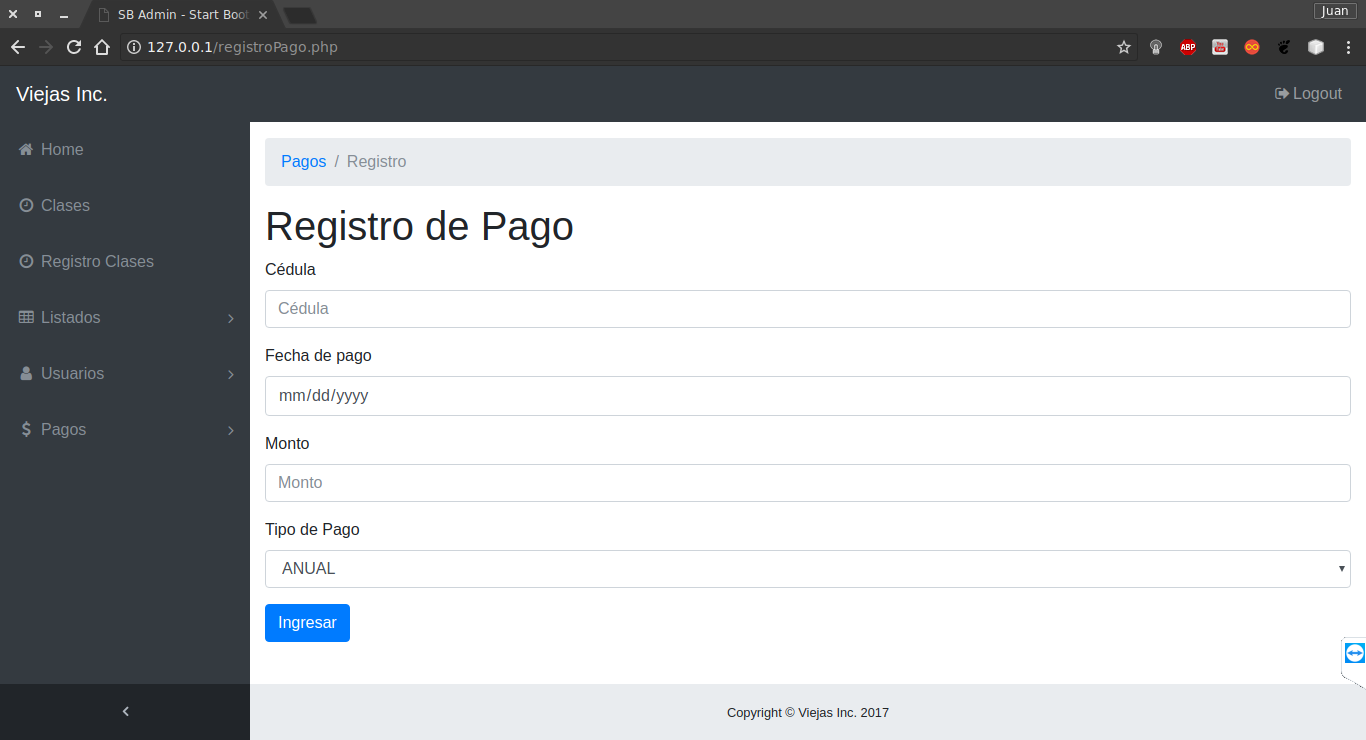
\includegraphics[width=\linewidth]{imagenes/pa_reg}
	\label{fig:pareg}
\end{figure}

\par Aquí se cargan los datos del pago (la fecha tiene el formato mes-dia-año), y la duración del pago, es decir, si es anual son 365 dias, si es semestral son 182 dias, y si es mensual son 31 dias.
\par Al presionar el botón ingresar aparecerá un mensaje de confirmación si el ingreso fue exitoso, de lo contrario un mensaje de error con el error en cuestión.

\subsection{Modificación}
\par Primero ir a la sección \verb|Pagos| en a barra de navegación, y dentro de esta sección elegir \verb|Registro Pago|. Esto desplegará la siguiente pantalla:
\begin{figure}[H]
	\centering
	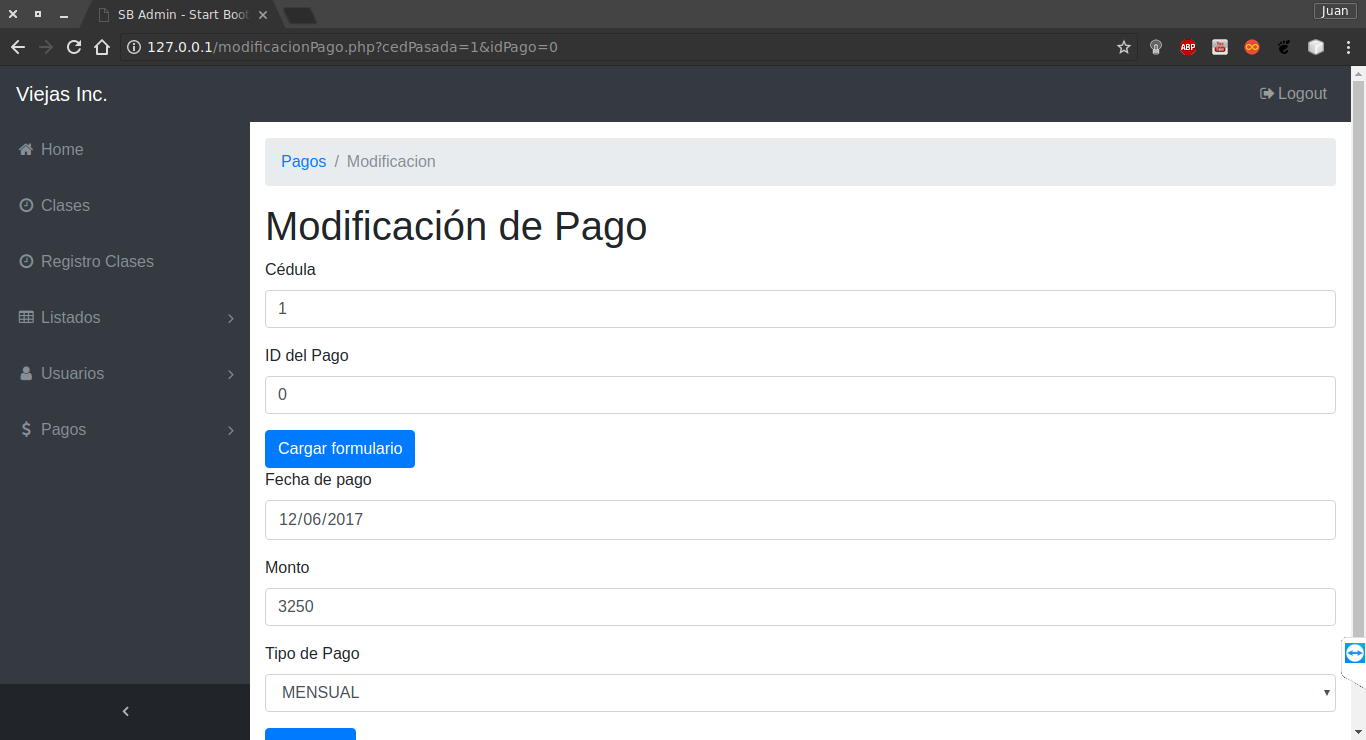
\includegraphics[width=\linewidth]{imagenes/pa_mod_car}
	\label{fig:pamodcar}
\end{figure}

\par Funciona igual que la modificación de usuario, solo que este es para los pagos realizados.
\subsection{Baja (lógica)}
\par Funciona igual que la baja de usuario, solo que a este hay que ingresarle la cédula del usuario y el id del pago correspondiente.
\subsection{Alta (lógica)}
\subsection{Baja (lógica)}
\par Funciona igual que la alta de usuario, solo que a este hay que ingresarle la cédula del usuario y el id del pago correspondiente.
\subsection{Listado}
\par Funciona igual que el listado de usuarios, solo que este al final del listado aparece la facturación mensual y anual(solo visible para administradores).
\begin{figure}[H]
	\centering
	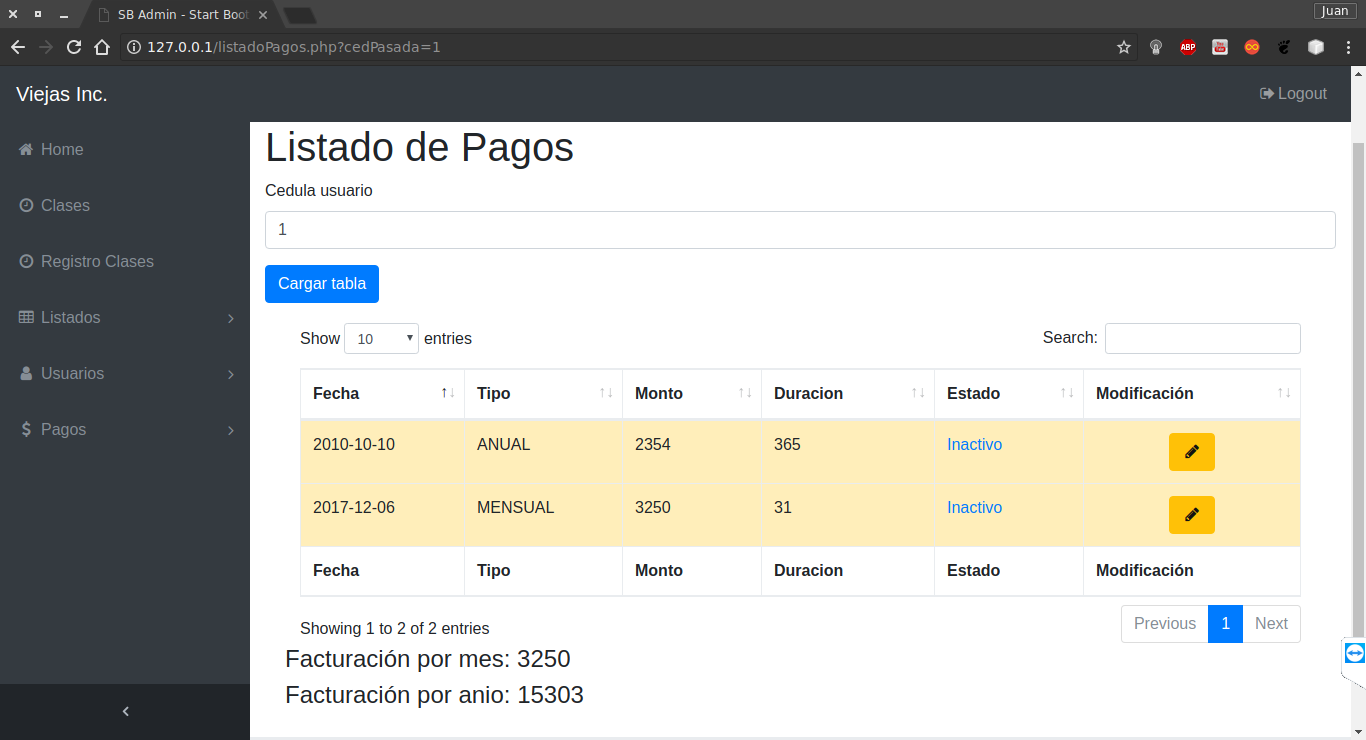
\includegraphics[width=\linewidth]{imagenes/pa_list_us}
	\label{fig:palistus}
\end{figure}

\newpage
\section{Clases}
En esta sección se indicará como llevar a cabo la administración de las actividades.
\subsection{Registro}
\par Para registrar una nueva clase/actividad, hay que ir a la sección \verb|Registro Clases|. Esto desplegará la siguiente pantalla:
\begin{figure}[H]
	\centering
	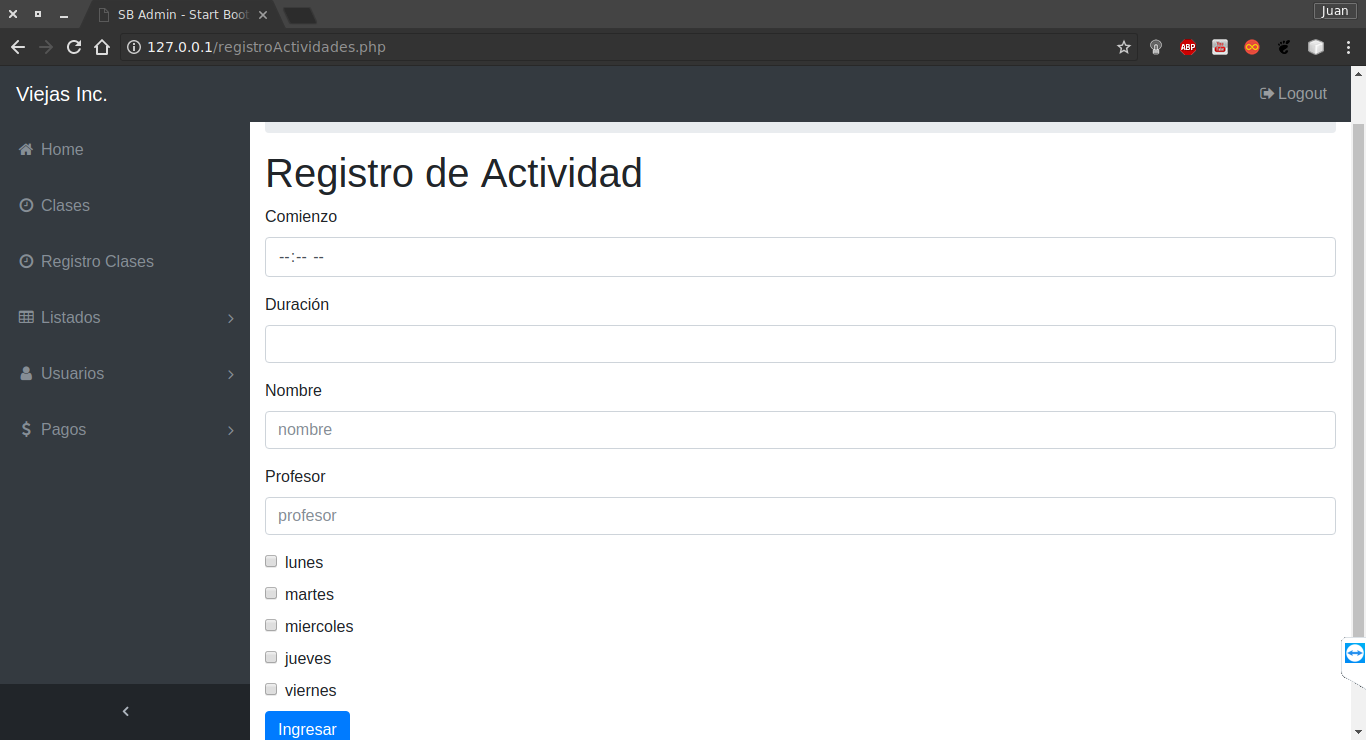
\includegraphics[width=\linewidth]{imagenes/ac_reg}
	\label{fig:acreg}
\end{figure}
\par El campo duración son los minutos que dura la clase, por ejemplo, si la actividad dura 1 hora, en duración se ingresa 60.
\par En los checkboxes se tildan los dias que se dictará la clase.
\par Para finalizar el ingreso de la actividad hay que presionar el botón ingresar. Luego aparecerá un mensaje de confirmación si el registro fue exitoso, de lo contrario aparecerá un mensaje con el error en cuestión.
\subsection{Listado}
\par Para obtener un listado de las clases, hay que ir a la sección clases. Esto desplegará la siguiente pantalla:
\begin{figure}[H]
	\centering
	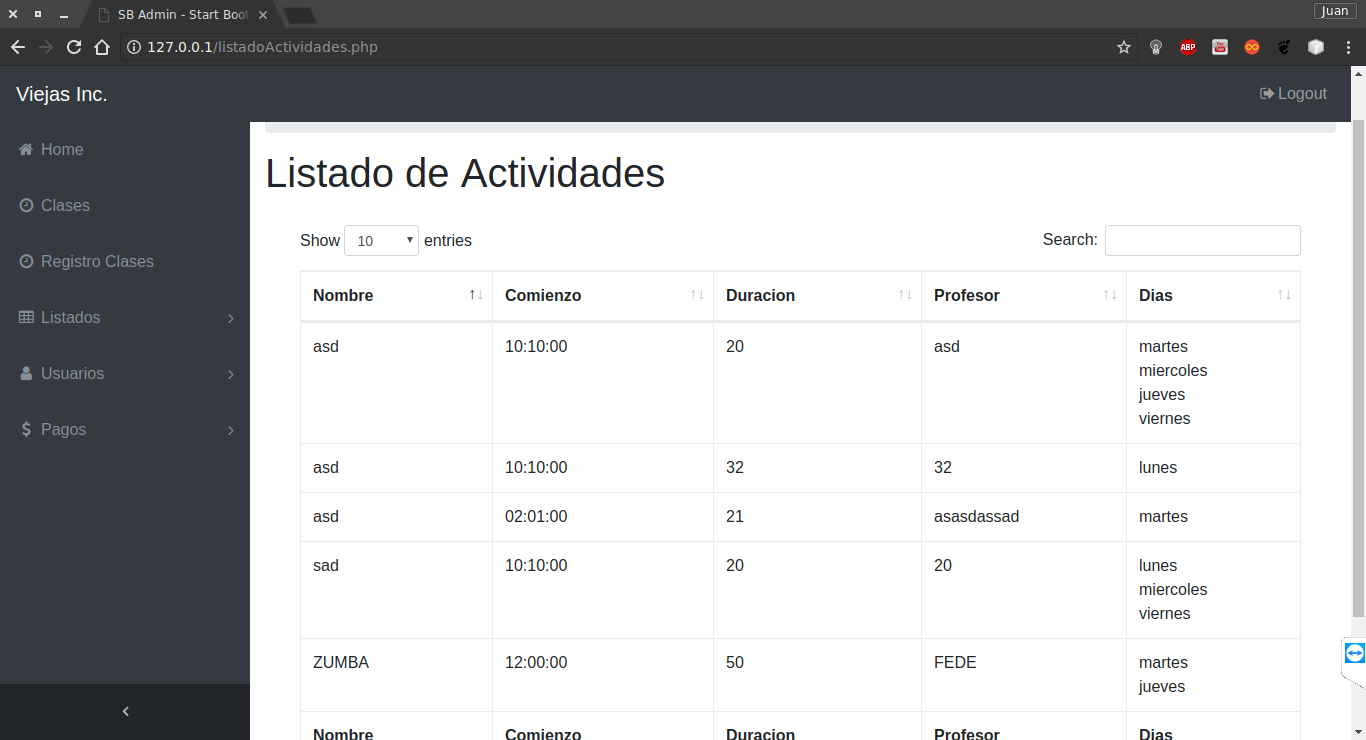
\includegraphics[width=\linewidth]{imagenes/ac_list}
	\caption{}
	\label{fig:aclist}
\end{figure}
\par Para la barra de búsqueda funciona igual que la de listado de usuarios y pagos.
\par Si se quiere filtrar los días de las actividades, hay que buscar ingresar el día en la barra de búsqueda.
\section{Página}
\subsection{Modificación}
\par Para modificar la página hay que ir a la sección \verb|Componentes| y elegir \verb|Pagina|. Esto despliega la siguiente pantalla:
\begin{figure}[H]
	\centering
	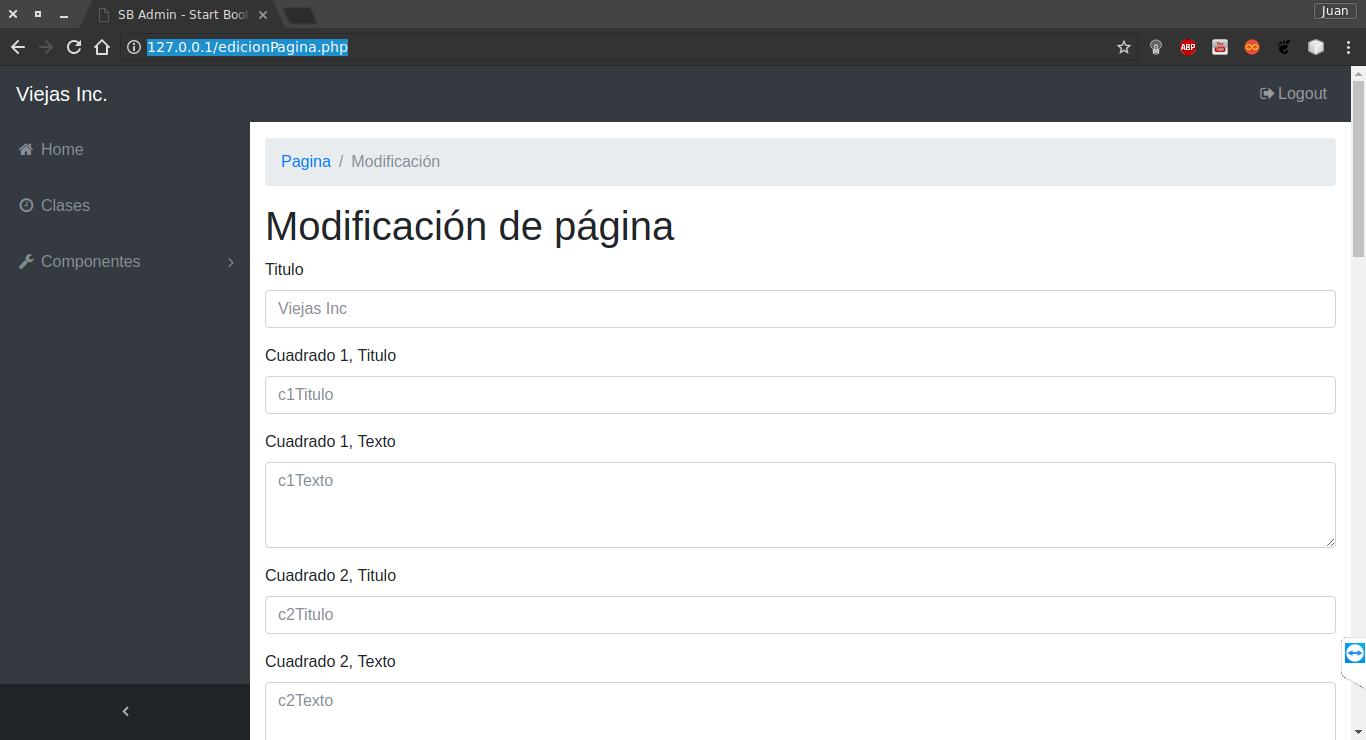
\includegraphics[width=\linewidth]{imagenes/mod_mod}
	\label{fig:modmod}
\end{figure}
Aquí se cargan los datos que se quiere que aparezcan en la página de inicio (Cambiar las imágenes no funciona).

\chapter{Modelo Entidad Relación}
\par Las tablas tienen más campos pero no me entraban en la imágen.

\begin{figure}[H]
	\centering
	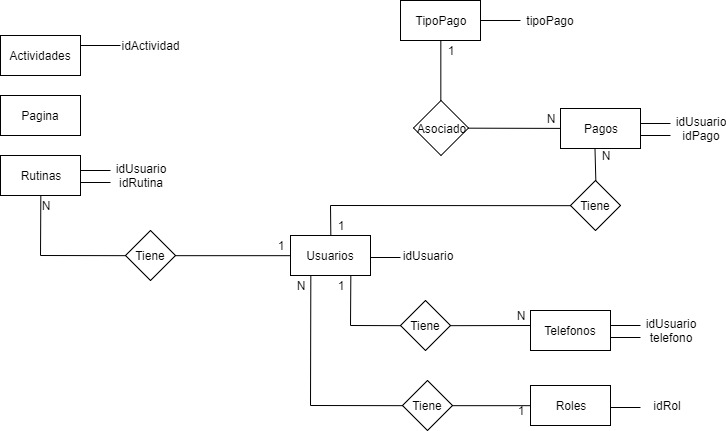
\includegraphics[width=\linewidth]{imagenes/mer}
	\label{fig:mer}
\end{figure}
\newpage
\begin{multicols}{3}
	\paragraph{Usuarios}
	\begin{itemize}
		\item idUsuario
		\item nombre
		\item apellido
		\item cedula
		\item direccion
		\item fechaNacimiento
		\item socMedica
		\item emerMovil
		\item antecedentes
		\item observaciones
		\item valido
		\item idRol
		\item contrasenia
	\end{itemize}
	
	\paragraph{Pagos}
	\begin{itemize}
		\item idUsuario
		\item idPago
		\item fechaPago
		\item tipoPago
		\item monto
		\item valido
	\end{itemize}
	\paragraph{Pagina}
	\begin{itemize}
		\item titulo
		\item c1Titulo
		\item c1Texto
		\item c2Titulo
		\item c2Texto
		\item c3Titulo
		\item c3Texto
		\item titulo2
		\item c4Titulo
		\item c4Texto
		\item c5Titulo
		\item c5Texto
		\item c6Titulo
		\item c6Texto
		\item fTitulo
		\item fTexto
		\item c1i
		\item c2i
		\item c3i
		\item c4i
		\item c5i
		\item c6i
	\end{itemize}
	\paragraph{TipoPago}
	\begin{itemize}
		\item tipoPago
		\item descripcion
		\item duracion
	\end{itemize}
	
	\paragraph{Actividades}
	\begin{itemize}
		\item idActividad
		\item comienzo
		\item duracion
		\item nombre
		\item profesor
		\item valido
		\item lunes
		\item martes
		\item miercoles
		\item jueves
		\item viernes
	\end{itemize}
\end{multicols}

\end{document}

